\documentclass[14pt,a4paper]{article}
\usepackage{mathtools}
\usepackage{amsmath}
\setcounter{MaxMatrixCols}{20}
\usepackage{setspace}
\usepackage{amsfonts}
\usepackage{graphicx}
\usepackage{geometry}
\geometry{a4paper, total = {210mm,297mm},left=35mm, right=25mm,top=25mm,bottom=25mm}
\usepackage{xcolor}
\usepackage[24pt]{mcode}
\usepackage{listings}

%Begin document - Midterm Project ME5554 - Applied Linear Systems

\begin{document}
\label{cover}
\begin{center}
	\vspace*{3cm}
	\large{\textbf{ME-5554 Applied Linear System \\ Midterm Project}}
	\vfill
	\textbf{Luan Cong Doan} \\ luandoan@vt.edu
	\vfill
	Nov 30, 2015
\end{center}
\pagebreak

The design engineer at Precision 3D Measuring Inc. have just developed a prototype 3D Coordinate Measuring Machine (CMM). In order to keep the cost low, the engineers have significantly reduced the amount of structural support in the frame, which unfortunately increase the compliance at the measurement probe. High compliance is generally not acceptable in a precision measurement system.\\

\begin{figure} [htp]
	\centering
	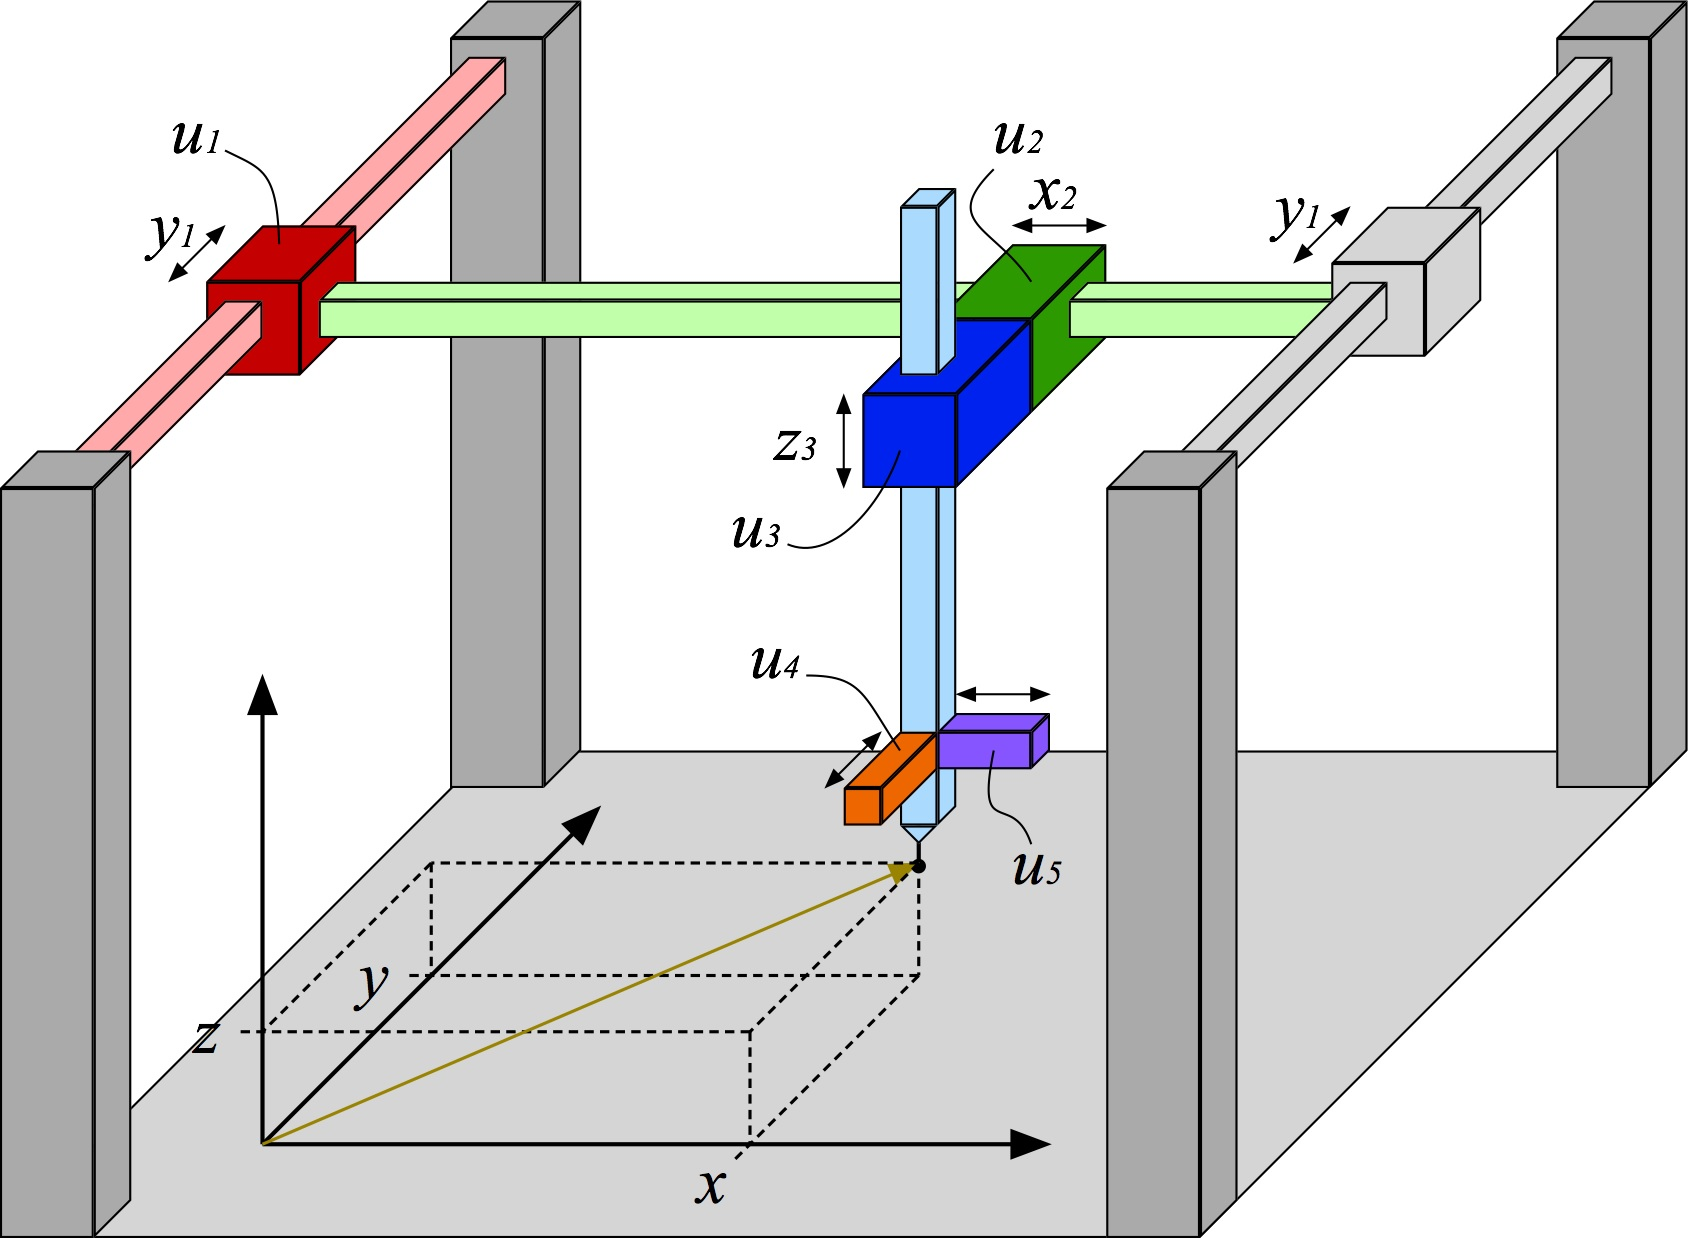
\includegraphics[scale=0.4]{MidtermProject.jpg}
	\caption{Prototype 3D Coordinate Measurement System}
\end{figure}

\large\textbf{Equation of Motion}\\
	The equation of motion for prototype CMM have already been derived and are given by the following equations:\\
	\doublespacing
	$ \hspace*{1cm} \dot{p}_1 = \alpha_1u_1 - \left(\dfrac{b_y}{M_y}\right)p_1 - \dot{p}_4   \hspace{3cm}  \dot{p}_5 = \alpha_2u_2 - \left(\dfrac{b_x}{M_x}\right)p_5 - \dot{p}_8 \\$
	$ \hspace*{1cm} \dot{q}_2 = \left(\dfrac{1}{M_y}\right)p_1 - \left(\dfrac{1}{m_4}\right)p_4 - \dot{q}_3   \hspace{2.2cm}  \dot{q}_6 = \left(\dfrac{1}{M_x}\right)p_5 - \left(\dfrac{1}{m_5}\right)p_8 - \dot{q}_7 $\\
	$ \hspace*{1cm} \dot{q}_3 = \left(\dfrac{1}{b_4}\right)\left(\alpha_4u_4 + \dot{p}_4 - k_4q_3\right)    \hspace{2.5cm}  \dot{q}_7 = \left(\dfrac{1}{b_5}\right)\left(\alpha_5u_5 + \dot{p}_8 - k_5q_7\right)$\\
	$ \hspace*{1cm} \dot{p}_4 = k_yq_2    \hspace{6.2cm}  \dot{p}_8 = k_xq_6 $\\
	$ \hspace*{1cm} \dot{y}_1 = \left(\dfrac{1}{M_y}\right)p_1    \hspace{5.2cm} \dot{x}_2 = \left(\dfrac{1}{M_x}\right)p_5 $\\
	$\hspace*{1cm} y = y_1 - q_2   \hspace{5.9cm} x = x_2 - q_6 $\\
	$ \hspace*{1cm} M_z\ddot{z} = -b_z\dot{z} + \alpha_3u_3 \\$

\pagebreak

\label{Problems}
\doublespacing
\large\textbf{Problem 1a.} Using the differential and algebraic equation of motion contruct a complete mathematical State-Space model for the dynamic system: \\
	State Space is defined: \\
	\hspace*{3cm}	$\dot{X} = A.X + B.U \\
	\hspace*{3.2cm}		Y = C.X + D.U $ \\
	We have: \\
	Define: \hspace{1cm} $ y_1 = p_9 \hspace{1.5cm} x_2 = q_{10} \hspace{1.5cm}  z = q_{11} \hspace{1.5cm} \dot{z} = p_{12}$ \\
	So: \\
	$ M_z\ddot{z} = -b_z\dot{z} + \alpha_3u_3  \Leftrightarrow M_z\dot{p}_{12} = -b_zq_{12} + \alpha_3u_3 \Leftrightarrow \dot{p}_{12} = -\dfrac{b_z}{M_z}q_{12} + \dfrac{\alpha_3}{M_z}u_3 $ \\
		
	\textbf{State variables:}  $X = {\begin{bmatrix}  p_1&q_2&q_3&p_4&p_5&q_6&q_7& p_8&p_9&q_{10}&q_{11}&p_{12} \end{bmatrix}}^T $ \\
	\hspace*{3.8cm} $\dot{X} = {\begin{bmatrix} \dot{p}_1 & \dot{q}_2 &\dot{q}_3 & \dot{p}_4 & \dot{p}_5 & \dot{q}_6 & \dot{q}_7 & \dot{p}_8 & \dot{p}_9 & \dot{q}_{10} & \dot{q}_{11} & \dot{p}_{12} \end{bmatrix}}^T $ \\
	1. 	$ \dot{p}_1 = \alpha_1u_1 - \left(\dfrac{b_y}{M_y}\right)p_1 - \dot{p}_4 = \alpha_1u_1 - \left(\dfrac{b_y}{M_y}\right)p_1 - k_yq_2 \\
	\hspace*{5.4cm} = \dfrac{b_y}{M_y}p_1 - k_yq_2 + \alpha_1u_1 $ \\
	2. $ \dot{q}_2 = \left(\dfrac{1}{M_y}\right)p_1 - \left(\dfrac{1}{m_4}\right)p_4 - \dot{q}_3 = \left(\dfrac{1}{M_y}\right)p_1 - \left(\dfrac{1}{m_4}\right)p_4 - \left(\dfrac{1}{b_4}\right)\left(\alpha_4u_4 + \dot{p}_4 - k_4q_3\right)\\
	\hspace*{5.9cm} = \dfrac{1}{M_y}p_1 - \dfrac{1}{m_4}p_4 + \dfrac{k_4}{b_4}q_3 - \dfrac{1}{b_4}k_yq_2 - \dfrac{\alpha_4}{b_4}u_4 \\
	\hspace*{5.9cm} = \dfrac{1}{M_y}p_1 - \dfrac{k_y}{b_4}q_2 + \dfrac{k_4}{b_4}q_3 - \dfrac{1}{m_4}p_4  - \dfrac{\alpha_4}{b_4}u_4 $ \\
	3. $ \dot{q}_3 = \left(\dfrac{1}{b_4}\right)\left(\alpha_4u_4 + \dot{p}_4 - k_4q_3\right) = \left(\dfrac{1}{b_4}\right)\left(\alpha_4u_4 + k_yq_2 - k_4q_3\right) \\
	\hspace*{5.8cm} = \dfrac{k_y}{b_4}q_2 - \dfrac{k_4}{b_4}q_3 + \dfrac{\alpha_4}{b_4}u_4 $ \\
	4. $ \dot{p}_4 = k_yq_2 $ \\
	5. $ \dot{p}_5 = \alpha_2u_2 - \left(\dfrac{b_x}{M_x}\right)p_5 - \dot{p}_8 = \alpha_2u_2 - \left(\dfrac{b_x}{M_x}\right)p_5 - k_xq_6  \\
	\hspace*{5.4cm} = -\dfrac{b_x}{M_x}p_5 - k_xq_6 + \alpha_2u_2 $\\
	6. $ \dot{q}_6 = \left(\dfrac{1}{M_x}\right)p_5 - \left(\dfrac{1}{m_5}\right)p_8 - \dot{q}_7 = \left(\dfrac{1}{M_x}\right)p_5 - \left(\dfrac{1}{m_5}\right)p_8 - \left(\dfrac{1}{b_5}\right)\left(\alpha_5u_5 + \dot{p}_8 - k_5q_7\right)\\
	\hspace*{5.9cm} = \dfrac{1}{M_x}p_5 - \dfrac{1}{m_5}p_8 + \dfrac{k_5}{b_5}q_7 - \dfrac{1}{b_5}k_xq_6 - \dfrac{\alpha_5}{b_5}u_5 \\
	\hspace*{5.9cm} = \dfrac{1}{M_x}p_5 - \dfrac{1}{b_5}k_xq_6 + \dfrac{k_5}{b_5}q_7 - \dfrac{1}{m_5}p_8 - \dfrac{\alpha_5}{b_5}u_5$ \\
	7. $ \dot{q}_7 = \left(\dfrac{1}{b_5}\right)\left(\alpha_5u_5 + \dot{p}_8 - k_5q_7\right) = \dfrac{1}{b_5}\left(\alpha_5u_5 + k_xq_6 - k_5q_7\right)\\
	\hspace*{5.7cm} = \dfrac{k_x}{b_5}q_6 - \dfrac{k_5}{b_5}q_7 + \dfrac{\alpha_5}{b_5}u_5 $\\
	8. $ \dot{p}_8 = k_xq_6 $ \\
	9. $ \dot{p}_9 = \dfrac{1}{M_y}p_1 $ \\
	10. $ \dot{q}_{10} = \dfrac{1}{M_x}p_5$ \\ 
	11. $ \dot{q}_{11} = p_{12} $ \\
	12. $ \dot{p}_{12} = -\dfrac{b_z}{M_z}p_{12} + \dfrac{\alpha_3}{M_z}u_3 $\\
	
		
	State equation: $ X = A.X + B.U $ \\
	Base on States variables we have State matrix A is determined: \\
	
	$ A = \begin{bmatrix} -\dfrac{b_y}{M_y} & -k_y & 0&0&0&0&0&0&0&0&0&0 \\ \dfrac{1}{M_y} & -\dfrac{k_y}{b_4} & \dfrac{k_4}{b_4} & -\dfrac{1}{m_4} &0&0&0&0&0&0&0&0 \\ 0& \dfrac{k_y}{b_4} & -\dfrac{k_4}{b_4} & 0&0&0&0&0&0&0&0&0 \\ 0 & k_y &0&0&0&0&0&0&0&0&0&0 \\ 0&0&0&0& -\dfrac{b_x}{M_x} & -k_x & 0&0&0&0&0&0 \\ 0&0&0&0& \dfrac{1}{M_x} & -\dfrac{k_x}{b_5} & \dfrac{k_5}{b_5} & -\dfrac{1}{m_5} & 0&0&0&0 \\ 0&0&0&0&0& \dfrac{k_x}{b_5} & -\dfrac{k_5}{b_5} & 0&0&0&0&0 \\ 0&0&0&0&0& k_x &0&0&0&0&0&0 \\ \dfrac{1}{M_y} &0&0&0&0&0&0&0&0&0&0&0 \\ 0&0&0&0 & \dfrac{1}{M_x} & 0&0&0&0&0&0&0 \\ 0&0&0&0&0&0&0&0&0&0&0&1 \\ 0&0&0&0&0&0&0&0&0&0&0& -\dfrac{b_z}{M_z}  \\  \end{bmatrix} $ \\
	
	\pagebreak
	Input matrix B: \\
	\hspace*{3cm} $ B = \begin{bmatrix} \alpha_1 & 0&0&0&0 \\ 0&0&0& -\dfrac{\alpha_4}{b_4} & 0 \\ 0&0&0&  \dfrac{\alpha_4}{b_4} & 0 \\ 0&0&0&0&0 \\ 0& \alpha_2 &0&0&0 \\ 0&0&0&0& -\dfrac{\alpha_5}{b_5} \\ 0&0&0&0 & \dfrac{\alpha_5}{b_5} \\ 0&0&0&0&0 \\ 0&0&0&0&0 \\ 0&0&0&0&0 \\ 0&0&0&0&0 \\ 0&0& \dfrac{\alpha_3}{M_z} &0&0 \end{bmatrix}$ \\
	
	
	Output equation: $ Y = C.X + D.U $\\
	Output states: $Y = {\begin{bmatrix}  x&y&z \end{bmatrix}}^T $ \\
	Output matrix C: \\
	\hspace*{2.5cm}$ C = \begin{bmatrix} 0&0&0&0&0& -1 &0&0&0& 1& 0& 0 \\ 0& -1 &0&0&0&0&0&0& 1 &0&0&0 \\ 0&0&0&0&0&0&0&0&0&0&1&0 \end{bmatrix} $ \\
	
	Direct Transmission matrix D: $D = [0]$ \\
	
	
	
\pagebreak

\large\textbf{Problem 1b.} Using the following numerical values to define an LTI object representation of above created state-space model in Matlab: \\
 $ M_y = 150 kg, \hspace{0.3cm}     M_x = 100 kg,  \hspace{0.3cm}   M_z = 50 kg,  \hspace{0.3cm}   b_y = 40 Ns/m,  \hspace{0.3cm}   b_x = 50 Ns/m, \\
 b_z = 10 Ns/m, \hspace{0.3cm}  k_x = 0.2 N/m,  \hspace{0.3cm}  m_4 = 20 kg,  \hspace{0.3cm}  b_4 = 2.51 Ns/m, \hspace{0.3cm} k_4 = 7.89 N/m, \\
 m_5 = 20 kg, \hspace{0.3cm} b_5 = 3.77 Ns/m, \hspace{0.3cm} k-5 = 7.89 N/m, \hspace{0.3cm} k_y = 0.1 N/m, \\
 \alpha_1 = 0.05 N/V, \hspace{0.3cm} \alpha_2 = 0.1 N/V,  \hspace{0.3cm} \alpha_3 = 0.1 N/V,  \hspace{0.3cm} \alpha_4 = 0.3 N/V, \hspace{0.3cm} \alpha_5 = 0.5 N/V $ \\

	With above values, we compute elements in matrices: \\
	\hspace*{2cm} $ \dfrac{b_y}{M_y} = \dfrac{40}{150} = 0.2667 \hspace{2cm} -k_y = -0.1$ \\
	\hspace*{2cm} $ \dfrac{1}{M_y} = \dfrac{1}{150} = 0.0067  \hspace{1.8cm} -\dfrac{k_y}{b_4} = -\dfrac{0.1}{2.51} = -0.0398 \\
	\hspace*{2.2cm} \dfrac{k_4}{b_4} = \dfrac{7.89}{2.51} = 3.1434  \hspace{2cm} -\dfrac{1}{m_4} = -\dfrac{1}{20} = -0.05 $ \\
	\hspace*{2cm} $ \dfrac{k_y}{b_4} = \dfrac{0.1}{2.51} = 0.0398  \hspace{1.8cm} -\dfrac{k_4}{b_4} = -\dfrac{7.89}{2.51} = -3.1434 $\\
	\hspace*{2cm} $ k_y = 0.1 $ \\
	\hspace*{2cm} $ \dfrac{b_x}{M_x} = \dfrac{50}{100} = 0.5 \hspace{2.4cm} -k_x = -0.2$ \\
	\hspace*{2cm} $ \dfrac{1}{M_x} = \dfrac{1}{100} = 0.01  \hspace{2.2cm} -\dfrac{k_x}{b_5} = -\dfrac{0.2}{3.77} = -0.0531 \\
	\hspace*{2.2cm} \dfrac{k_5}{b_5} = \dfrac{7.89}{3.77} = 2.0928  \hspace{2cm} -\dfrac{1}{m_5} = -\dfrac{1}{20} = -0.05 $ \\
	\hspace*{2cm} $ \dfrac{k_x}{b_5} = \dfrac{0.2}{3.77} = 0.0531  \hspace{2cm} -\dfrac{k_5}{b_5} = -\dfrac{7.89}{3.77} = -2.0928 $\\
	\hspace*{2cm} $ k_x = 0.2 $ \\
	\hspace*{2cm} $ \dfrac{b_z}{M_z} = \dfrac{10}{50} = 0.2 $ \\
	\hspace*{2cm} $ \dfrac{1}{M_x} = \dfrac{1}{100} = 0.01 $ \\
	\hspace*{2cm} $ \dfrac{1}{M_y} = \dfrac{1}{150} = 0.0067 $ \\
	
	\hspace*{2cm} $ \alpha_1 = 0.05 \hspace{4cm} \dfrac{\alpha_4}{b_4} = \dfrac{0.3}{2.51} = 0.1195 $ \\
	\hspace*{2.5cm} $ \alpha_2 = 0.1 \hspace{4.3cm} \dfrac{\alpha_5}{b_5} = \dfrac{0.5}{3.77} = 0.1326 $ \\
	\hspace*{2.5cm} $ \dfrac{\alpha_3}{M_z} = \dfrac{0.1}{50} = 0.002 $ \\

	\pagebreak
	We have: \\
	State matrix: \\
	$ A = \begin{bmatrix} -0.2667 & -0.1 & 0&0&0&0&0&0&0&0&0&0 \\ 0.0067 & -0.0398 & 3.1434 & -0.05 &0&0&0&0&0&0&0&0 \\ 0& 0.0398 & -3.1434 & 0&0&0&0&0&0&0&0&0 \\ 0 & 0.1 &0&0&0&0&0&0&0&0&0&0 \\ 0&0&0&0& -0.5 & -0.2 & 0&0&0&0&0&0 \\ 0&0&0&0& 0.01 & -0.0531 & 2.0928 & -0.05 & 0&0&0&0 \\ 0&0&0&0&0& 0.0531 & -2.0928 & 0&0&0&0&0 \\ 0&0&0&0&0& 0.2 &0&0&0&0&0&0 \\ 0.0067 &0&0&0&0&0&0&0&0&0&0 \\ 0&0&0&0& 0.01 &0&0&0&0&0&0 &0 \\ 0&0&0&0&0&0&0&0&0&0&0&1 \\ 0&0&0&0&0&0&0&0&0&0&0& -0.2 \end{bmatrix} $ \\
	
	Input matrix B: \\
	\hspace*{2cm} $ B = \begin{bmatrix} 0.05 &0&0&0&0 \\ 0&0&0& -0.1195 & 0 \\ 0&0&0& 0.1195 & 0 \\ 0&0&0&0&0 \\ 0& 0.1 &0&0&0 \\ 0&0&0&0& -0.1326 \\ 0&0&0&0 & 0.1326 \\ 0&0&0&0&0 \\ 0&0&0&0&0 \\ 0&0&0&0&0 \\ 0&0&0&0&0 \\ 0&0& 0.002 &0&0 \end{bmatrix}$ 
	
	\begin{lstlisting}
	% State input matrix
	A = [-0.2667 -0.1 0 0 0 0 0 0 0 0 0 0; 0.0067 -0.0398 3.1434 -0.05 0 0 0 0 0 0 0 0; 
	0 0.0398 -3.1434 0 0 0 0 0 0 0 0 0; 0 0.1 0 0 0 0 0 0 0 0 0 0;
	0 0 0 0 -0.5 -0.2 0 0 0 0 0 0; 0 0 0 0 0.01 -0.0531 2.0928 -0.05 0 0 0 0;
	0 0 0 0 0 0.0531 -2.0928 0 0 0 0 0; 0 0 0 0 0 0.2 0 0 0 0 0 0;
	0.0067 0 0 0 0 0 0 0 0 0 0 0; 0 0 0 0 0.01 0 0 0 0 0 0 0;
	0 0 0 0 0 0 0 0 0 0 0 1; 0 0 0 0 0 0 0 0 0 0 0 -0.2];
	
	% Input matrix
	B = [0.05 0 0 0 0; 0 0 0 -0.12 0; 0 0 0 0.12 0; 0 0 0 0 0; 0 0.1 0 0 0; 0 0 0 0 -0.133;
	0 0 0 0 0.133; 0 0 0 0 0; 0 0 0 0 0; 0 0 0 0 0; 0 0 0 0 0; 0 0 0.002 0 0];
	
	% Output matrix
	C = [0 0 0 0 0 -1 0 0 0 1 0 0; 0 -1 0 0 0 0 0 0 1 0 0 0; 0 0 0 0 0 0 0 0 0 0 1 0];
	
	D = [];		% Transmisstion matrix
	
	% Creating State-space model:
	SYS = ss(A,B,C,D);
	
	% Define statename, inputname and outputname
	states = {'st1','st2','st3','st4','st5','st6','st7','st8','st9','st10','st11','st12'};
	inputs = {'in1','in2','in3','in4','in5'};
	outputs = {'out1','out2','out3'};
	set(SYS,'statename',states);
	set(SYS,'inputname',inputs);
	set(SYS,'outputname',outputs);
	\end{lstlisting}
	Result for Problem 1b: 
	\begin{lstlisting}
	>> SYS
	
	SYS =
	
	a = 
	st1      st2      st3      st4      st5      st6      st7      st8      st9     st10     st11     st12
	st1   -0.2667     -0.1        0        0        0        0        0        0        0        0        0        0
	st2    0.0067  -0.0398    3.143    -0.05        0        0        0        0        0        0        0        0
	st3         0   0.0398   -3.143        0        0        0        0        0        0        0        0        0
	st4         0      0.1        0        0        0        0        0        0        0        0        0        0
	st5         0        0        0        0     -0.5     -0.2        0        0        0        0        0        0
	st6         0        0        0        0     0.01  -0.0531    2.093    -0.05        0        0        0        0
	st7         0        0        0        0        0   0.0531   -2.093        0        0        0        0        0
	st8         0        0        0        0        0      0.2        0        0        0        0        0        0
	st9    0.0067        0        0        0        0        0        0        0        0        0        0        0
	st10        0        0        0        0     0.01        0        0        0        0        0        0        0
	st11        0        0        0        0        0        0        0        0        0        0        0        1
	st12        0        0        0        0        0        0        0        0        0        0        0     -0.2
	
	b = 
	in1     in2     in3     in4     in5
	st1     0.05       0       0       0       0
	st2        0       0       0   -0.12       0
	st3        0       0       0    0.12       0
	st4        0       0       0       0       0
	st5        0     0.1       0       0       0
	st6        0       0       0       0  -0.133
	st7        0       0       0       0   0.133
	st8        0       0       0       0       0
	st9        0       0       0       0       0
	st10       0       0       0       0       0
	st11       0       0       0       0       0
	st12       0       0   0.002       0       0
	
	c = 
	st1   st2   st3   st4   st5   st6   st7   st8   st9  st10  st11  st12
	out1     0     0     0     0     0    -1     0     0     0     1     0     0
	out2     0    -1     0     0     0     0     0     0     1     0     0     0
	out3     0     0     0     0     0     0     0     0     0     0     1     0
	
	d = 
	in1  in2  in3  in4  in5
	out1    0    0    0    0    0
	out2    0    0    0    0    0
	out3    0    0    0    0    0
	
	Continuous-time state-space model.
		
	\end{lstlisting}
	
\pagebreak
\large\textbf{Problem 1c.} Use the MINREAL function in Matlab to demonstrate whether your LTI state-space model is a minimum realization or not.
	\begin{lstlisting}
	sysr = minreal(SYS);
	if (size(sysr) == size(SYS))
	fprintf('LTI system is minimum realization.\n');
	else
	fprintf('LTI system is not minimum realization.\n');
	end
	\end{lstlisting}
	Result of checking:
	\begin{lstlisting}
	LTI system is minimum realization.
	\end{lstlisting}
\pagebreak
\large\textbf{Problem 2:} Demonstrate that this open-loop system is Completely Controllable. 
	\begin{lstlisting}
	Co = ctrb(SYS);     % calculate the control matrix
	r = rank(Co);       % calculate rank of matrix
	testC = size(A,1);
	if r == testC
	fprintf('System is Completely Controllable.\n');
	else
	fprintf('System is not completely controllable.\n');
	end
	\end{lstlisting}
	Result of checking controllability:
	\begin{lstlisting}
	System is Completely Controllable.
	\end{lstlisting}
	
	Subset of control inputs checking:
	\begin{lstlisting}
	for i = 1:4
		if rank(ctrb(SYS(:,[1:i]))) == testC
			fprintf('Subset of control inputs could get %d inputs.\n',i);
			SYS(:,[1:i])
		end
	end
	\end{lstlisting}
	Results:
	\begin{lstlisting}
	Subset of control inputs could get 3 inputs.
	
	ans =
	
	a = 
	st1      st2      st3      st4      st5      st6      st7      st8      st9     st10     st11     st12
	st1   -0.2667     -0.1        0        0        0        0        0        0        0        0        0        0
	st2    0.0067  -0.0398    3.143    -0.05        0        0        0        0        0        0        0        0
	st3         0   0.0398   -3.143        0        0        0        0        0        0        0        0        0
	st4         0      0.1        0        0        0        0        0        0        0        0        0        0
	st5         0        0        0        0     -0.5     -0.2        0        0        0        0        0        0
	st6         0        0        0        0     0.01  -0.0531    2.093    -0.05        0        0        0        0
	st7         0        0        0        0        0   0.0531   -2.093        0        0        0        0        0
	st8         0        0        0        0        0      0.2        0        0        0        0        0        0
	st9    0.0067        0        0        0        0        0        0        0        0        0        0        0
	st10        0        0        0        0     0.01        0        0        0        0        0        0        0
	st11        0        0        0        0        0        0        0        0        0        0        0        1
	st12        0        0        0        0        0        0        0        0        0        0        0     -0.2
	
	b = 
	in1    in2    in3
	st1    0.05      0      0
	st2       0      0      0
	st3       0      0      0
	st4       0      0      0
	st5       0    0.1      0
	st6       0      0      0
	st7       0      0      0
	st8       0      0      0
	st9       0      0      0
	st10      0      0      0
	st11      0      0      0
	st12      0      0  0.002
	
	c = 
	st1   st2   st3   st4   st5   st6   st7   st8   st9  st10  st11  st12
	out1     0     0     0     0     0    -1     0     0     0     1     0     0
	out2     0    -1     0     0     0     0     0     0     1     0     0     0
	out3     0     0     0     0     0     0     0     0     0     0     1     0
	
	d = 
	in1  in2  in3
	out1    0    0    0
	out2    0    0    0
	out3    0    0    0
	
	Continuous-time state-space model.
	
	Subset of control inputs could get 4 inputs.
	
	ans =
	
	a = 
	st1      st2      st3      st4      st5      st6      st7      st8      st9     st10     st11     st12
	st1   -0.2667     -0.1        0        0        0        0        0        0        0        0        0        0
	st2    0.0067  -0.0398    3.143    -0.05        0        0        0        0        0        0        0        0
	st3         0   0.0398   -3.143        0        0        0        0        0        0        0        0        0
	st4         0      0.1        0        0        0        0        0        0        0        0        0        0
	st5         0        0        0        0     -0.5     -0.2        0        0        0        0        0        0
	st6         0        0        0        0     0.01  -0.0531    2.093    -0.05        0        0        0        0
	st7         0        0        0        0        0   0.0531   -2.093        0        0        0        0        0
	st8         0        0        0        0        0      0.2        0        0        0        0        0        0
	st9    0.0067        0        0        0        0        0        0        0        0        0        0        0
	st10        0        0        0        0     0.01        0        0        0        0        0        0        0
	st11        0        0        0        0        0        0        0        0        0        0        0        1
	st12        0        0        0        0        0        0        0        0        0        0        0     -0.2
	
	b = 
	in1    in2    in3    in4
	st1    0.05      0      0      0
	st2       0      0      0  -0.12
	st3       0      0      0   0.12
	st4       0      0      0      0
	st5       0    0.1      0      0
	st6       0      0      0      0
	st7       0      0      0      0
	st8       0      0      0      0
	st9       0      0      0      0
	st10      0      0      0      0
	st11      0      0      0      0
	st12      0      0  0.002      0
	
	c = 
	st1   st2   st3   st4   st5   st6   st7   st8   st9  st10  st11  st12
	out1     0     0     0     0     0    -1     0     0     0     1     0     0
	out2     0    -1     0     0     0     0     0     0     1     0     0     0
	out3     0     0     0     0     0     0     0     0     0     0     1     0
	
	d = 
	in1  in2  in3  in4
	out1    0    0    0    0
	out2    0    0    0    0
	out3    0    0    0    0
	
	Continuous-time state-space model.
	\end{lstlisting}
	
\pagebreak
\large\textbf{Problem 3:} Compute the open loop poles of this system, the natural frequencies with unit of Hz, and the damping ratios for each eigenvalues.
	\begin{lstlisting}
	Char = poly(A);          % define characteristic equation from state matrix
	Poles = roots(Char);     % compute system poles
	Eigs = eig(A);           % compute eigenvalues of state matrix
	[wn,zeta] = damp(SYS);  % compute natural frequency and damping ratio of system
	
	Wn = wn/(2*pi);          % convert natural frequency to unit of Hz
	Zeta = abs(zeta);        
	
	column = [1:12];
	Values = column';
	table(Values, Wn, Zeta, Eigs, Poles)    % print out the table of values with Wn ascending
	\end{lstlisting}
	Result:
	\begin{lstlisting}
	Values       Wn         Zeta              Eigs                   Poles        
	______    ________    ________    ____________________    ____________________
	
	1               0           1             0+0i                    0+0i       
	2               0           1             0+0i                    0+0i       
	3               0           1       -3.1832+0i                    0+0i       
	4        0.011233    0.016702    -0.0011788+0.070567i       -3.1832+0i       
	5        0.011233    0.016702    -0.0011788-0.070567i       -2.1458+0i       
	6        0.015777    0.019661      -0.26436+0i             -0.49625+0i       
	7        0.015777    0.019661       -2.1458+0i             -0.26436+0i       
	8        0.031831           1      -0.49625+0i                 -0.2+0i       
	9        0.042075           1     -0.001949+0.099112i     -0.001949+0.099112i
	10         0.07898           1     -0.001949-0.099112i     -0.001949-0.099112i
	11         0.34151           1             0+0i           -0.0011788+0.070567i
	12         0.50662           1          -0.2+0i           -0.0011788-0.070567i
	\end{lstlisting}
\pagebreak

\large\textbf{Problem 4:} Simulate the open-loop response of the system for three seconds, assuming all initial states are zero except for non-zero IC's defined below.\\
$ \hspace*{2cm} y_1(0) = 0.5, \hspace{2cm}        p_1(0) = 300   \hspace{2cm}   z(0) = 0.7 $\\
$\hspace*{2cm} x_2(0) 0.6 \hspace{2.7cm}      p_5(0) = - 150  \hspace{1.7cm}   \dot{z}(0) = - 0.09348 $ 
	\begin{lstlisting}
	X40 = [300; 0; 0; 0; -150; 0; 0; 0; 0.5; 0.6; 0.7; -0.09348];  % initial states for problem 4
	figure;
	[y,t,x] = initial(SYS,X40,3);          % apply initial function for 3 seconds
	plot(t, y(:,1),'r',t,y(:,2),'b',t,y(:,3),'g');
	title('Response for Initial Condition in 3 seconds');
	xlabel('time');
	ylabel('output');
	legend('Output1 - X','Output2 - Y', 'Output3 - Z');
	print('ResponseForInitialCondition','-dpng');   % save plot as an image
	\end{lstlisting}
	Result: 
	\begin{figure}[htp]
		\begin{center}
			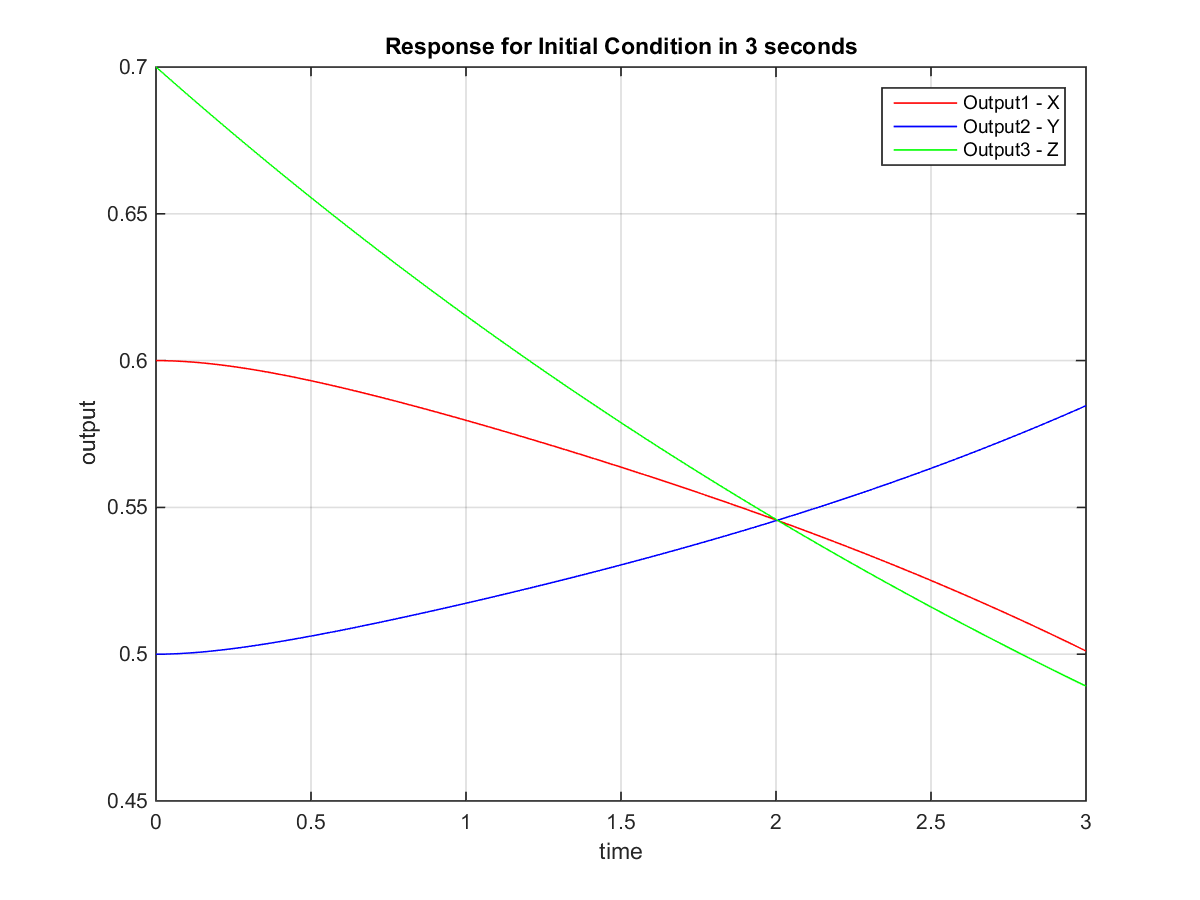
\includegraphics[scale = 0.7]{ResponseForInitialCondition.png}
		\end{center}
		\caption{Response for Initial Condition in 3 seconds}
	\end{figure}\\
\pagebreak
	
\large\textbf{Problem 5:} Design a full-state feedback controller that meets the following performance requirements:
	\begin{enumerate}
		\item Each ouput must be within $\pm 1 cm$, after 8 seconds
		\item $|u_1| \leq 1000, \hspace{0.5cm}|u_2| \leq 1000, \hspace{0.5cm} |u_3| \leq 200, \hspace{0.5cm} |u_4| \leq 100, \hspace{0.5cm} |u_5| \leq 100$
	\end{enumerate}
	Simulate the closed-loop response of the system for ten second, assuming all initial states are zero except for the non-zero IC's defined bellow:\\
	\hspace*{2cm} $y_1(0) = 1 \hspace{2cm} x_2(0) = 1 \hspace{2cm} z(0) = 1$
	
	\begin{lstlisting}
	% Poles 1
	Poles1 = Poles;      % using poles from original state matrix A
	G1 = place(A,B,Poles1);       % compute Gain matrix from Poles of open-loop
	
	Ac1 = A - B*G1;            % compute state matrix for close-loop
	B1 = [];              % new B matrix is 0
	SYSC1 = ss(Ac1,B1,C,D);    % new close-loop system
	
	%Checking step:
	figure;
	[yc1,tc1,xc1] = initial(SYSC1,X50,10);
	plot(tc1,yc1);
	grid on; legend('y1','y2','y3');
	
	U1 = -G1*xc1';          % new control input space base on gain G
	figure;
	plot(tc1,U1);         % plot and check control inputs
	grid on; legend('u1','u2','u3','u4','u5');
	print('FullStateFeedback','-dpng');
	
	% Poles 2
	Poles2 = [-0.001 + 0.0001i; -0.001 - 0.0001i;  -0.002 + 0.015i; -0.002 - 0.015i; -2.5 + 0.0001i; -2 - 0.025i;
	-0.5 + 0.001i; -0.65 - 0.001i; -0.2 + 0.0325i; -0.2 - 0.0325i; -0.0012 + 0.008i; -0.0012 - 0.008i];
	
	G2 = place(A,B,Poles2);
	Ac2 = A - B*G2;
	B2 = [];
	sysc2 = ss(Ac2, B2, C,D);
	
	[yc2,tc2,xc2] = initial(sysc2,X50,10);
	figure;
	plot(tc2,yc2);
	grid on; legend('y1','y2','y3');
	
	U2 = -G2*xc2';
	figure;
	plot(tc2,U2);   grid on; legend('u1','u2','u3','u4','u5');
	
	% Poles 3
	Poles3 = [-0.001 + 0.0001i; -0.001 - 0.0001i;  -0.002 + 0.015i; -0.002 - 0.015i; -2.5 + 0.0001i; -2 - 0.025i;
	-0.5 + 0.001i; -0.65 - 0.001i; -0.2 + 0.0325i; -0.2 - 0.0325i; -0.0015 + 0.006i; -0.0015 - 0.008i];
	G3 = place(A,B,Poles3);
	Ac3 = A - B*G3;
	B3 = [];
	sysc3 = ss(Ac3, B3, C,D);
	
	[yc3,tc3,xc3] = initial(sysc3,X50,10);
	figure;
	plot(tc3,yc3);
	grid on; legend('y1','y2','y3');
	U3 = -G3*xc3';
	figure;
	plot(tc3,U3);
	grid on; legend('u1','u2','u3','u4','u5');
	
	% Poles 4
	Poles4 = [-0.001 + 0.0001i; -0.001 - 0.0001i;  -0.002 + 0.015i; -0.002 - 0.015i; -2.5 + 0.0001i; -2 - 0.025i;
	-0.5 + 0.001i; -0.65 - 0.001i; -0.2 + 0.0325i; -0.2 - 0.0325i; -0.0018 + 0.0065i; -0.0015 - 0.008i];
	G4 = place(A,B,Poles4);
	Ac4 = A - B*G4;
	B4 = [];
	sysc4 = ss(Ac4, B4, C,D);
	
	[yc4,tc4,xc4] = initial(sysc4,X50,10);
	figure;
	plot(tc4,yc4);
	grid on; legend('y1','y2','y3');
	U4 = -G4*xc4';
	figure;
	plot(tc4,U4);
	grid on; legend('u1','u2','u3','u4','u5');
	
	% Poles 5
	Poles5 = [-0.001 + 0.0001i; -0.001 - 0.0001i;  -0.002 + 0.015i; -0.002 - 0.015i; -2.5 + 0.0001i; -2 - 0.025i;
	-0.5 + 0.001i; -0.65 - 0.001i; -0.2 + 0.0325i; -0.2 - 0.0325i; -0.0017 + 0.0055i; -0.0015 - 0.008i];
	G5 = place(A,B,Poles5);
	Ac5 = A - B*G5;
	B5 = [];
	sysc5 = ss(Ac5, B5, C,D);
	
	[yc5,tc5,xc5] = initial(sysc5,X50,10);
	figure;
	plot(tc5,yc5);
	grid on; legend('y1','y2','y3');
	U5 = -G5*xc5';
	figure;
	plot(tc5,U5);
	grid on; legend('u1','u2','u3','u4','u5');
	
	%% Print out
	figure;
	subplot(15,2,7);
	plot(tc5,yc5(:,1),'r');
	xlabel('Time'); ylabel('Output');
	grid on; title('First Output');
		subplot(15,2,17);
	plot(tc5,yc5(:,2),'b');
	xlabel('Time'); ylabel('Output');
	grid on; title('Second Output');
		subplot(15,2,27);
	plot(tc5,yc5(:,3),'g');
	xlabel('Time'); ylabel('Output');
	grid on; title('Third Output');
		subplot(15,2,6);
	plot(tc5,U5(1,:),'r');
	xlabel('Time'); ylabel('Control Input 1');
	grid on; title('First Control Input');
		subplot(15,2,12);
	plot(tc5,U5(2,:),'r');
	xlabel('Time'); ylabel('Control Input 2');
	grid on; title('Second Control Input');
		subplot(15,2,18);
	plot(tc5,U5(3,:),'r');
	xlabel('Time'); ylabel('Control Input 3');
	grid on; title('Third Control Input');
		subplot(15,2,24);
	plot(tc5,U5(4,:),'r');
	xlabel('Time'); ylabel('Control Input 4');
	grid on; title('Forth Control Input');
		subplot(15,2,30);
	plot(tc5,U5(5,:),'r');
	xlabel('Time'); ylabel('Control Input 5');
	grid on; title('Fifth Control Input');
		print('FeedbackSystem','-dpng');
	
	\end{lstlisting}
	Full-State feedback system base on Poles 5:
	\begin{figure}[htp]
		\begin{center}
			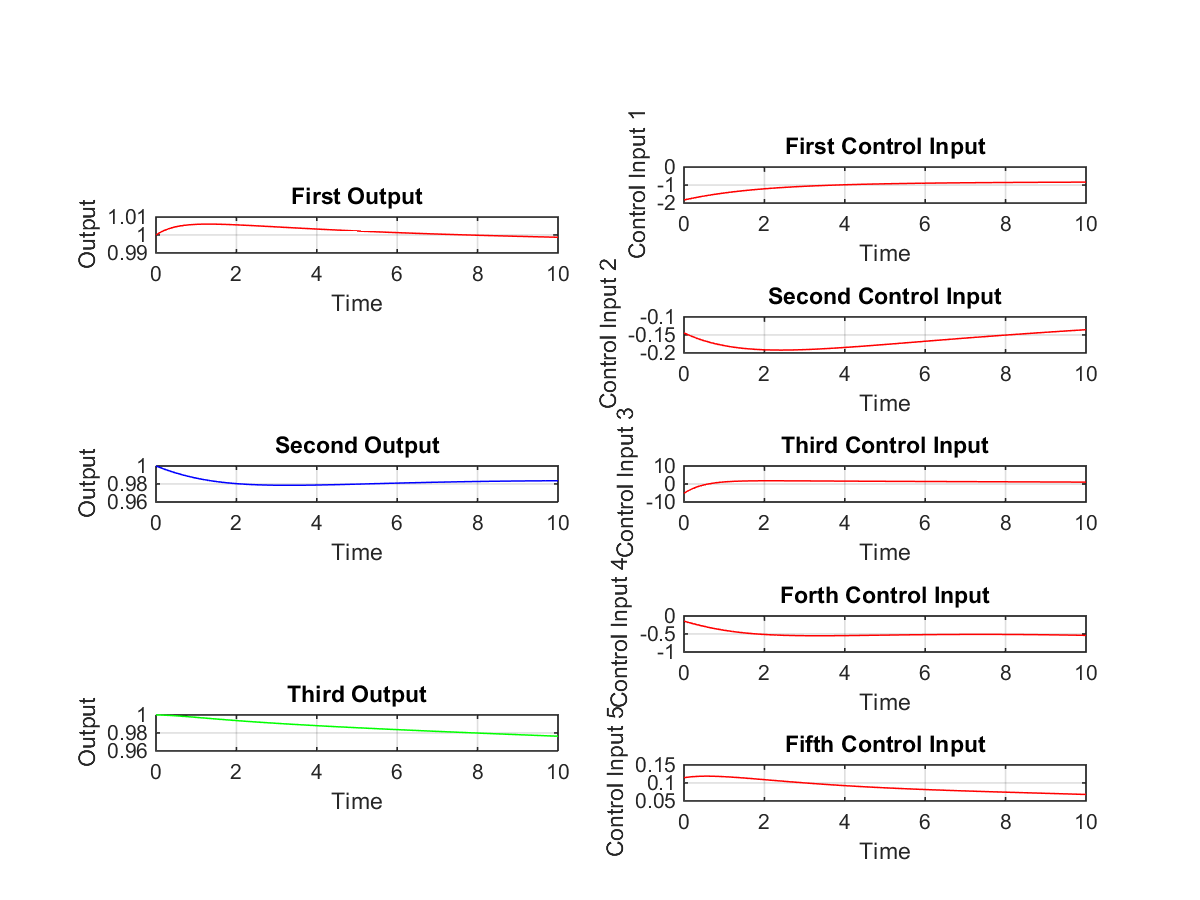
\includegraphics[scale = 0.8]{FeedbackSystem.png}
		\end{center}
		\caption{Full State Feedback System for 10 seconds}
	\end{figure}

\end{document}